\section{\Large PROBLEM SET 2}
\subsection{PROBLEM 1}
\textit{Define orbit initial conditions and make sure you can propagate the orbit of the satellite over multiple orbits using either a Keplerian propagator or a numerical integration scheme (see AA279A material). Best would be to use a numerical integrator, so that you can later try to feed the same environmental forces for orbit propagation which are applied for attitude propagation (very cool!).}

From the science users' handbook, we obtain the following orbital elements \cite{NISARHandbook}.

\begin{table}[H]
\begin{tabular}{lllllll}
\textbf{OE} & \textit{a} & \textit{e} & \textit{i} & \textit{$\Omega$} & \textit{$\omega$} & \textit{$\nu$} \\ \hline
\textbf{Value} & 7125.48662 km & 0.0011650 & 98.40508$\degree$ & -19.61601$\degree$ & 89.99764$\degree$ & -89.99818$\degree$
\end{tabular}
\end{table}

We convert these using a MATLAB function into ECI coordinates that can be fed into a numerical orbital propagator. Notice that we first convert the orbital elements a, e, and $\nu$ into perifocal (PQW) coordinates, using a and e to find the semi-latus rectum and a, e, and $\nu$ to find the distance to the central body (Earth). Then, we perform a series of rotations on these coordinates parameterized by $\omega$, i, and $\Omega$ to obtain new coordinates in the ECI frame.

\lstinputlisting{src/oe2eci.m}

Then, we can numerically propagate in MATLAB using \texttt{ode113} using a function that computes the time derivative of the ECI state. This is accomplished simply by setting the time derivative of position equal to the velocity portion of the state and setting the time derivative of velocity equal to an acceleration computed using the law of universal gravitation. Note that while our propagator does not include disturbance forces, it will be easy to incorporate these later. See the appendix corresponding to Problem Set 2 for application of \texttt{ode113}.

\lstinputlisting{src/propagator.m}

Now, we plot the trajectory for one orbit in Figure \ref{fig:simple_propagator}.

\begin{figure}[H]
\centering
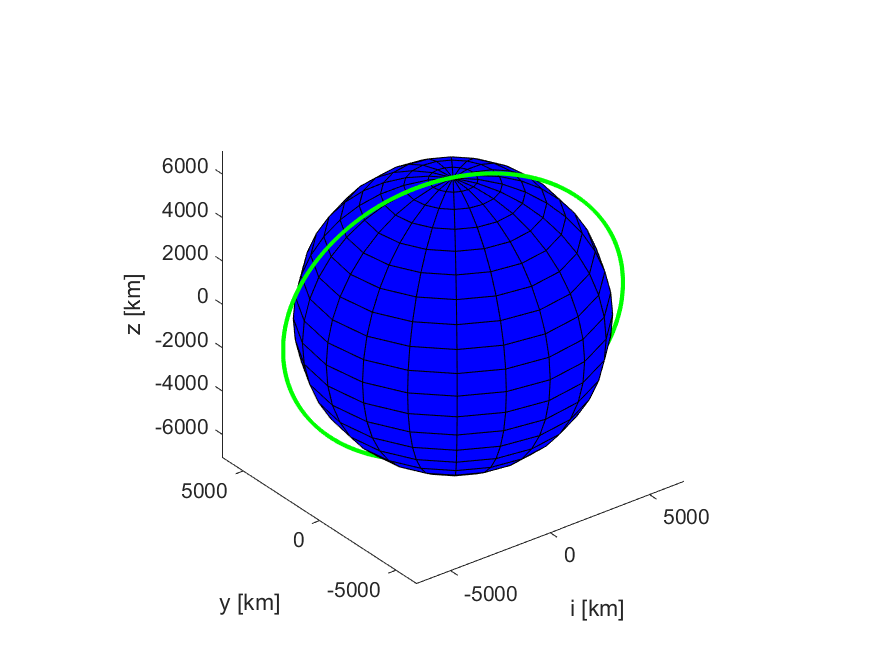
\includegraphics[scale=0.75]{Images/ps2_problem1.png}
\caption{A single orbit for NISAR in ECI coordinates (no perturbations)}
\label{fig:simple_propagator}
\end{figure}


\subsection{PROBLEM 2}
\textit{In general the body axes are not the principal axes. Identify principal axes through the eigenvector/eigenvalue problem discussed in class and compute the rotation matrix from body to principal axes.}
% This step: find eigenvalues and eigenvectors, where eigenvalues specify the principal axes inertia tensor and the eigenvectors specify the rotation
% KUSAL


\subsection{PROBLEM 3}
\textit{At this stage you should have a simple 3D model of your spacecraft including geometry and mass properties of each element. This includes at least two coordinate systems, body and principal axes respectively, and the direction cosine matrix between them. Plot axes of triads in 3D superimposed to spacecraft 3D model.}

\begin{figure}[H]
\centering
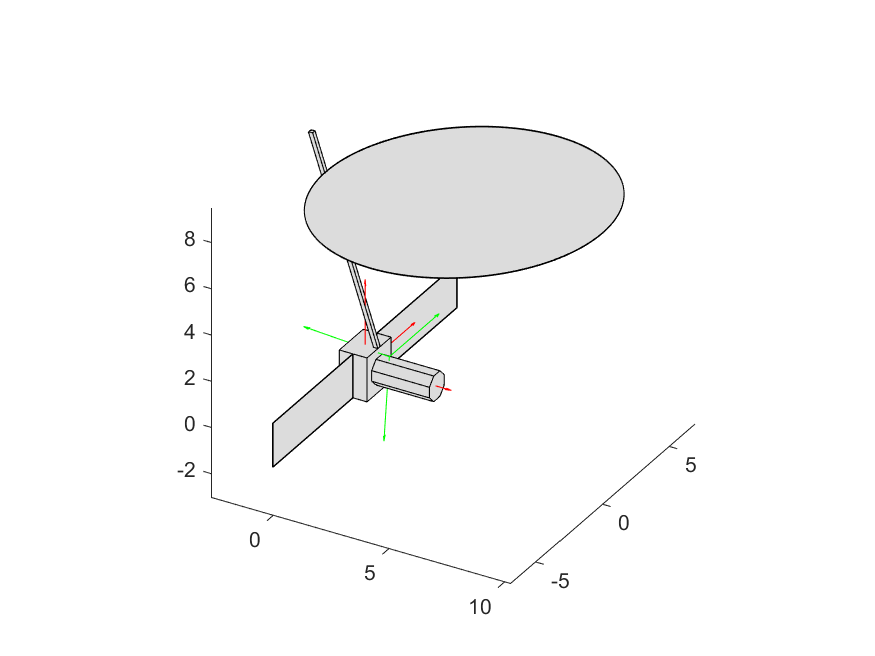
\includegraphics[scale=0.75]{Images/ps2_model.png}
\caption{Principal axes at center of mass (green) and body axes at origin (red)}
\label{fig:ps2_model}
\end{figure}


\subsection{PROBLEM 4}
\textit{Program Euler equations in principal axes (e.g. in Matlab/Simulink). No external torques.}

\lstinputlisting{src/eulerPropagator.m}


\subsection{PROBLEM 5}
\textit{Numerically integrate Euler equations from arbitrary initial conditions ($\omega<\qty{10}{\degree/\second}$, $\omega_{i}\neq0$). Multiple attitude revolutions.}


\subsection{PROBLEM 6}
\textit{Plot rotational kinetic energy and momentum ellipsoids in 3D (axis equal) corresponding to chosen initial conditions. Verify that semi-axis of ellipsoids corresponds to theoretical values.}


\subsection{PROBLEM 7}
\textit{Plot polhode in same 3D plot. Verify that it is the intersection between the ellipsoids.}


\subsection{PROBLEM 8}
\textit{Plot polhode in three 2D planes identified by principal axes (axis equal). Verify that shapes of resulting conic sections correspond to theory.}


\subsection{PROBLEM 9}
\textit{Repeat above steps changing initial conditions, e.g. setting angular velocity vector parallel to principal axis. Is the behavior according to expectations?}